\chapter{手搖手工皂}

\section{實驗原理}
動物脂肪和植物油主要成份是由長鏈脂肪酸(fatty acids)和甘油所反應而成的酯類。這些三酸甘油酯(triglyceride or triacylglycerol)經過水解反應會產生甘油和脂肪酸鹽。因為脂肪酸鈉鹽是離子化合物,如果濃度很低時,它是溶在水中的,但是如果高濃度的脂肪酸鈉鹽,它會聚集在一起而凝集形成了肥皂。基本上,酯類的水解反應被稱為皂化(saponification),其反應式如圖所示,其中R為長鏈的飽和或不飽和的烴基。

\begin{figure}[H]
\centering
\graphicspath{{chemistry/}}
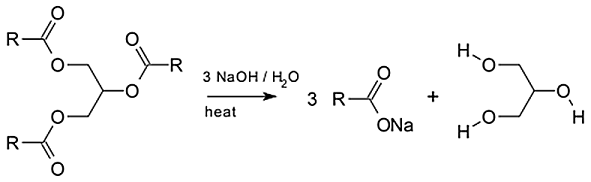
\includegraphics[width=\textwidth, center]{fatty.png}
\caption{皂化反應} \vskip 10 pt
\label{fig:soap}
\end{figure}

\section{實驗器材及藥品}
\begin{table}[H]
\centering
\begin{tabular}{|c|c|}
\hline
\textbf{實驗器材} & \textbf{實驗藥品} \\ \hline
\begin{tabular}[c]{@{}c@{}}空寶特瓶罐X1\\   磅秤 數個\\   秤量紙 數張\\   燒杯X2\\   玻棒X1\\   空紙杯X1\end{tabular} & \begin{tabular}[c]{@{}c@{}}NaOH 7g\\   $\rm KOH$ 10g\\   $\rm H_{2}O$ 46.3g\\   棕櫚油 50g\\   紅色染料\\   黃色染料\\   玫瑰水\end{tabular} \\ \hline
\end{tabular}
\end{table}

\section{實驗步驟}
\begin{enumerate}
\item 秤出7g NaOH 和10g KOH
\item 用燒杯裝 43.6g $\rm H_{2}O$,並將秤好的NaOH和KOH倒入燒杯並溶解
\item 在寶特瓶內裝入50g棕櫚油並加入步驟2配好的溶液
\item 鎖緊瓶蓋,搖晃瓶身直到混和液變濃稠
\item 之後可加入玫瑰水和染料並到入空紙杯,等待一個禮拜即可
\end{enumerate}